\documentclass{article}
\usepackage{fancyhdr}
\usepackage{extramarks}
\usepackage{amsmath}
\usepackage{amsthm}
\usepackage{amsfonts}
\usepackage{tikz}
\usepackage[plain]{algorithm}
\usepackage{algpseudocode}

\begin{document}
\author{Chuan Lu}
\title{BIOS:7600 Homework 5}
\maketitle

\medskip

\begin{enumerate}

\item Problem 3.1

The plot for two-stage adaptive lasso is shown in Figure \ref{3.1}, where the inital estimate of $\beta$ is the OLS solution. The fit plot is generated by \texttt{ncvreg}.

\begin{figure}[h]
\centering
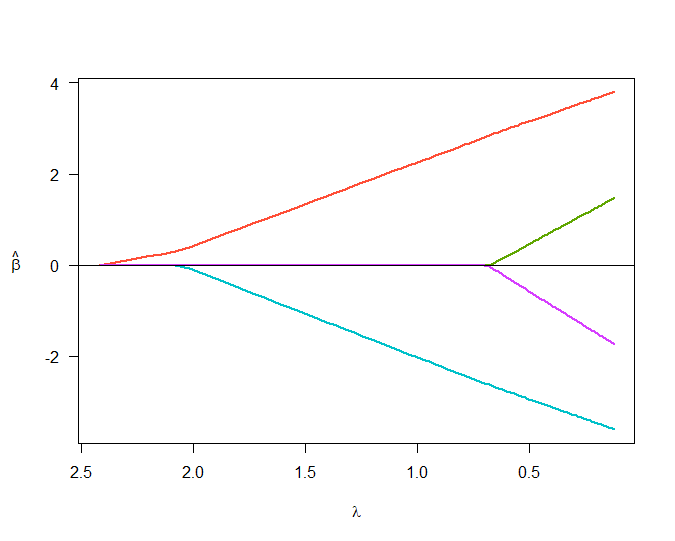
\includegraphics[scale=0.5]{two_stage_lasso.png}
\caption{two stage adaptive lasso}
\label{3.1}
\end{figure}

Since the weights are constant across all values of $\lambda$, the path looks different with pathwise adaptive lasso, but similar with original lasso paths, but all four variables are selected with a smaller $\lambda$ since the initial weights are 1.231007,  2.067553, 1.310293, 2.252761, larger than 1 used in lasso.

\item Problem 3.2(b)

\begin{proof}
First, when $|x| \le \lambda$, SCAD penalty is just the $\lVert\cdot\rVert_1 $ penalty for lasso, so the thresholding operator is the same with lasso. When $|x| \ge \gamma\lambda$, the penalty is a constant, so the operator does not change the value. Now consider the case when $2\lambda < z < \gamma\lambda$; the other part when $z < 0$ is just the same. The subgradient of $Q$ in the univariate problem is
$$
\partial Q = -z +\beta + \frac{\gamma\lambda - \partial(|\beta|)}{\gamma - 1}.
$$
If $\beta \ne 0$, then let $\partial Q = 0$, we have 
$$
\beta = \frac{\gamma-1}{\gamma-2}(z-\frac{\lambda\gamma}{\gamma-1}).
$$
If $\beta = 0$, then $\partial(|\beta|)= [-1, 1] $, and by $0\in\partial Q$ we have
$$
|z| \le \frac{\gamma\lambda}{\gamma-1}.
$$
So
$$
\beta = \left\{
\begin{aligned}
\frac{\gamma-1}{\gamma-2}(z-\frac{\lambda\gamma}{\gamma-1}), & \quad |z| > \frac{\gamma\lambda}{\gamma-1}, \\
0, & \quad \text{otherwise}.
\end{aligned}
\right.
$$
Notice $\gamma > 2$, we have $\frac{\gamma}{\gamma-1} < 2$. By combining the second case with the lasso operator, we can show the result.
\end{proof}

\item Problem 2.7
\begin{proof}
First, the lasso approximation is 
$$
f(y_i) = x_i^\top S(\beta_i\mid \lambda) = x_i^\top S(\frac{1}{n}x_i^\top y),
$$
which is piecewise linear and continuous. Then $f$ is Lipschitz, which means $f$ is absolutely continuous. Besides,
$$
f'(y) = \frac{1}{n}x^\top x \cdot 1_{|\beta| > \lambda} = \frac{1}{n} I_n\cdot 1_{|\beta^{OLS}| > \lambda}, 
$$
which is bounded, so
$$
df = \sum_{i=1}^{n} f'(y_i) = \sum_{i=1}^{n} 1_{|\beta^{OLS}_i| > \lambda},
$$
which proves the result.

\end{proof}

\item Problem 3.3

\begin{enumerate}
\item 
By the same process with the last problem, we get
$$
f'(y) = \left\{
\begin{aligned}
&0, &\quad  |\beta^{OLS}| < \lambda \\
&\frac{\gamma}{\gamma-1}, &\quad  \lambda \le |\beta^{OLS}| \le \gamma\lambda \\
&1, &\quad  |\beta^{OLS}| > \gamma\lambda
\end{aligned}
\right.
$$
Then
$$
df = \sum_{i=1}^{n}f'(y_i) = \#\{|\beta^{OLS}| > \gamma\lambda\} +\frac{\gamma}{\gamma-1} \#\{\lambda \le |\beta^{OLS}| \le \gamma\lambda\}.
$$

\item 
When $\gamma = 3$, 
$$
df_{MCP} = \#\{|\beta^{OLS}| > 3\lambda\} +\frac{3}{2} \#\{\lambda \le |\beta^{OLS}| \le 3\lambda\} \ge df_{LASSO}.
$$

\end{enumerate}

\item Problem 3.7

\begin{table}[h]
\centering
\begin{tabular}{|l|l|l|l|l|l|}
\hline
  & forward   & lasso     & ridge     & MCP       & SCAD      \\ \hline
1 & 0.3645032 & 0.1436703 & 0.6538278 & 0.1218058 & 0.1318939 \\ \hline
2 & NA        & 0.1680950 & 2.0420509 & 0.1434068 & 0.1540713 \\ \hline
3 & 0.7072784 & 0.8207570 & 0.6495371 & 0.7677788 & 0.7481251 \\ \hline
4 & NA        & 2.258974  & 2.028072  & 2.178437  & 2.140876  \\ \hline
\end{tabular}
\end{table}



\item Problem 3.8

\begin{enumerate}
\item The plot is show in Figure \ref{3.8}.
\begin{figure}[h]
\centering
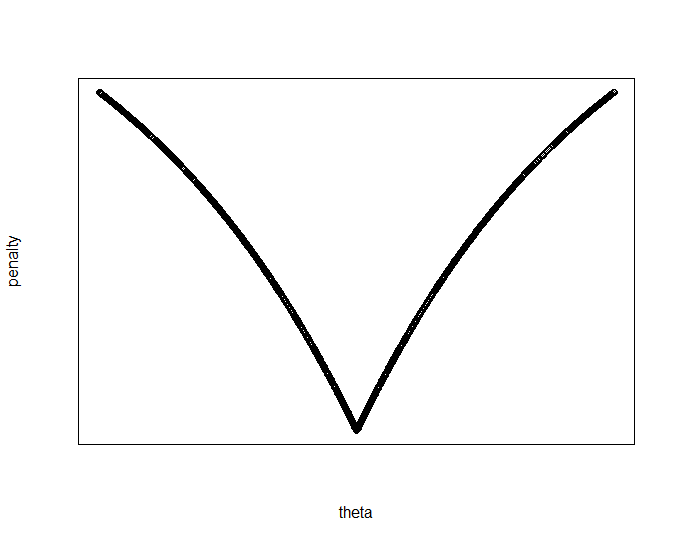
\includegraphics[scale=0.5]{exponential_penalty.png}
\caption{exponential penalty}
\label{3.8}
\end{figure}

\item 
The graph of $p'$ is shown in Figure \ref{3.8.2}, where $p'$ is
$$
p'(\theta) = \left\{
\begin{aligned}
&e^{-\frac{\tau}{\lambda}\theta}, &\quad |\theta| > 0 \\
&[-1, 1], &\quad |\theta| = 0
\end{aligned}
\right.
$$
\begin{figure}[ht]
\centering
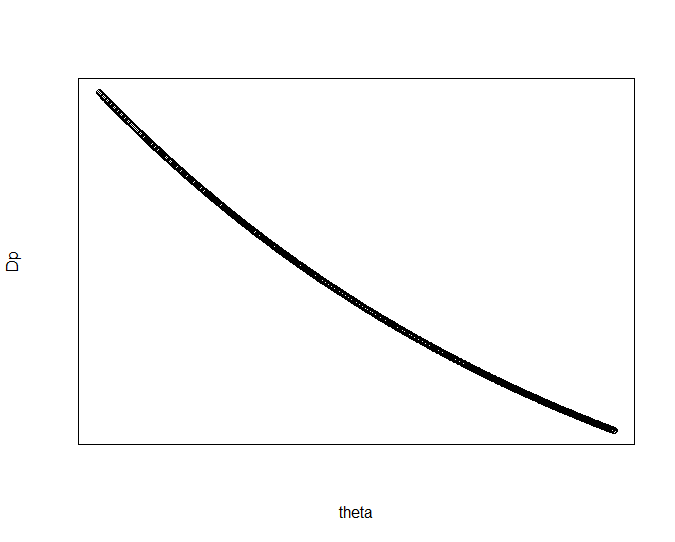
\includegraphics[scale=0.5]{d_exponential_penalty.png}
\caption{derivative of exponential penalty}
\label{3.8.2}
\end{figure}

\item Based on the result of $p'$, the estimates would be similar with MCP when $\beta $ is not large; however, when $\beta$ is large, since $p' > 0$, it should be a combination of MCP and Lasso, while MCP has a larger weight.

\item TBD.

\end{enumerate}

\item Problem 3.10

$\gamma = 2.3$ by minimizing \texttt{fit\$cve}.

\begin{enumerate}
\item 
The plots of $R^2 $ by MCP and Lasso are shown in Figure \ref{3.10.1}. The max $R^2 $ by MCP is about 0.5, while it is about 0.25.

\begin{figure}[ht]
\centering
\vbox{
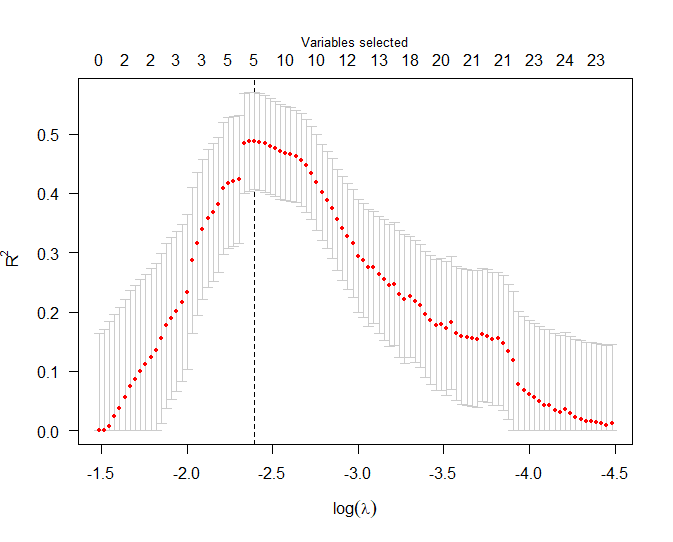
\includegraphics[scale=0.3]{Rsquare_MCP.png}
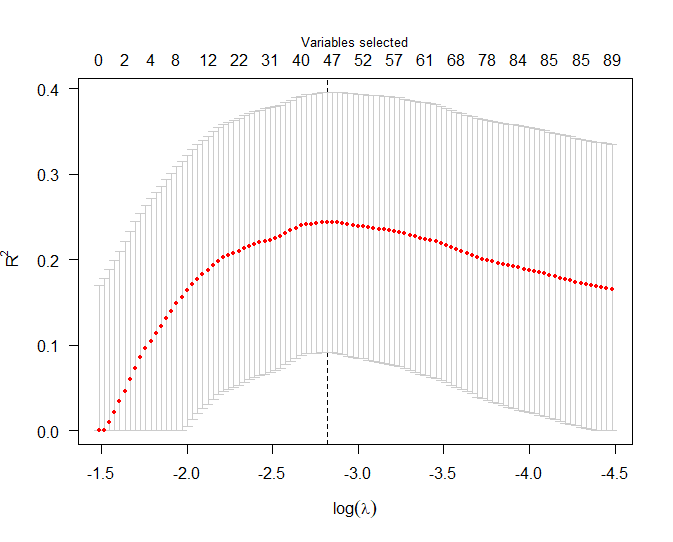
\includegraphics[scale=0.3]{Rsquare_Lasso.png}
}
\caption{Estimates of $R^2 $ with MCP (left) and Lasso (right).}
\label{3.10.1}
\end{figure}

\item 
At the max $R^2 $, 5 variables are chosen from MCP, while 47 variables are chosen from lasso.

\item 
The gene enters MCP model first is \texttt{C16ORF30}, enters lasso first is \texttt{GNPDA1}. I think there must be something wrong with the code since the genes are different. The paths are shown in Figure \ref{3.10.2}:

\begin{figure}[ht]
\centering
\vbox{
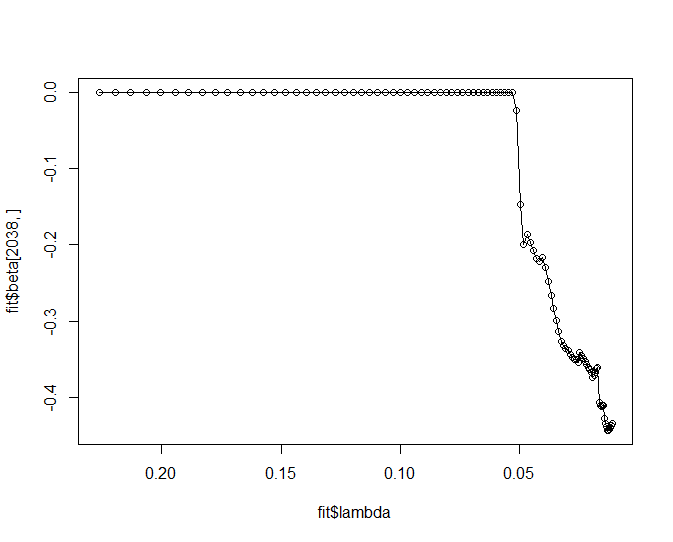
\includegraphics[scale=0.3]{path_MCP.png}
\includegraphics[scale=0.3]{path_Lasso.png}
}
\caption{Fitting paths with MCP (left) and Lasso (right).}
\label{3.10.2}
\end{figure}

\end{enumerate}

\end{enumerate}


\end{document}